\documentclass[12pt]{beamer}

% Theme & Colors
\usetheme{Madrid} % Try: Berlin, Copenhagen, CambridgeUS, Warsaw...
\usecolortheme{dolphin} % Try: seahorse, crane, beaver...

% Encoding & Fonts
\usepackage[utf8]{inputenc}
\usepackage[T1]{fontenc}
\usepackage{lmodern} % Better font
\usepackage{luatexja}
\usepackage{luatexja-fontspec}
\usepackage{amsmath,amssymb,mathtools,ascmac,amsthm,amscd,tikz-cd}
\usetikzlibrary{arrows.meta,calc,quotes,angles}
\setmainjfont{Noto Sans CJK JP}

% Title Information
\newcommand{\circnum}[2][]{%
  \tikz[baseline=(n.base)] \node (n) [circnum,#1]{#2};%
}
\title[]{三角形の辺と角の関係}
\date{\today}

\begin{document}
% Title Page
\begin{frame}
  \titlepage
\end{frame}

% Outline
\begin{frame}{}
  \tableofcontents
\end{frame}

% Section 1
\section{三角形の成立条件}
\begin{frame}{}
  \begin{block}{三角形の成立条件}
		3つの正の数$a,b,c$に対して,3辺の長さが$a,b,c$である三角形の存在条件は,
\[a + b > c,\quad b+c > a,\quad c+a > b.\]
  \end{block}
	\begin{center}
	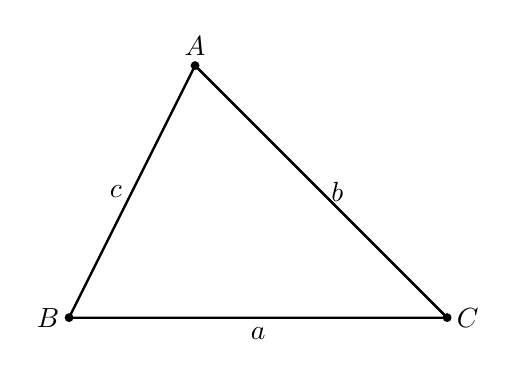
\begin{tikzpicture}[scale=1.6]
  % Define the vertices
  \coordinate (B) at (0,0);
  \coordinate (C) at (3,0);
  \coordinate (A) at (1,2);
  % Draw the triangle
  \draw[thick] (A)--(B)--(C)--cycle;
	\draw[thick] (A)--(B) node[midway,left] {$c$};
	\draw[thick] (B)--(C) node[midway,below] {$a$};
	\draw[thick] (C)--(A) node[midway,right] {$b$};
  \fill (A) circle (1pt) node[above] {$A$};
  \fill (B) circle (1pt) node[left] {$B$};
  \fill (C) circle (1pt) node[right] {$C$};
\end{tikzpicture}
\end{center}
\bullet 寄り道すると遠い.
\end{frame}

\begin{frame}{}
  \begin{block}{三角形の成立条件}
		3つの正の数$a,b,c$に対して,3辺の長さが$a,b,c$である三角形の存在条件は,
\[a + b > c,\quad b+c > a,\quad c+a > b.\]
  \end{block}
	すべての式を$a$について解くと,
\[c- b < a ,\quad a < b + c,\quad b - c < a.\]
まとめて,	
\[ |b - c| < a < b + c.\]
\end{frame}

\section{辺と比の関係}
\begin{frame}{}
	\begin{block}{定理9}
	三角形\triangle ABC において,次が成り立つ.
		\[b < c \Longleftrightarrow \angle B < \angle C.\]
	\end{block}
\begin{center}
	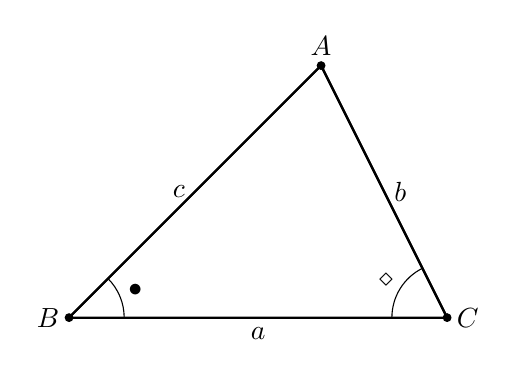
\begin{tikzpicture}[scale=1.6]
  % Define the vertices
  \coordinate (B) at (0,0);
  \coordinate (C) at (3,0);
  \coordinate (A) at (2,2);
  % Draw the triangle
  \draw[thick] (A)--(B)--(C)--cycle;
	\draw[thick] (A)--(B) node[midway,left] {$c$};
	\draw[thick] (B)--(C) node[midway,below] {$a$};
	\draw[thick] (C)--(A) node[midway,right] {$b$};
  \fill (A) circle (1pt) node[above] {$A$};
  \fill (B) circle (1pt) node[left] {$B$};
  \fill (C) circle (1pt) node[right] {$C$};
	 \path pic["$\bullet $",draw,angle radius=7mm,angle eccentricity=1.3] {angle = C--B--A};
	 \path pic["$\diamond $",draw,angle radius=7mm,angle eccentricity=1.3] {angle = A--C--B};
\end{tikzpicture}
\end{center}
\end{frame}

\end{document}
